% Appendix A

\chapter{3D structural models} % Main appendix title

\label{AppendixB} % For referencing this appendix elsewhere, use \ref{AppendixA}

\lhead{Appendix B. \emph{3D structural models}} % This is for the header on each page - perhaps a shortened title

The arbitrary complex 3D nanostructured targets can be generated by graphical softwares beforehand and traced by two types of sophisticated 3D structural algorithms in IM3D code, that is, CSG and FETM methods\cite{Li2:2011,Li:2013}. Then the different types of targets are set in the corresponding coordinate systems as shown in Fig.\ref{Fig.2}, respectively. The ion beams with different atomic numbers and incident directions follow different types of space-distributions (i.e., specified point, center point, uniform or Gaussian random distributions and so on). The targets are considered as composing of different geometric elements each of which with different amorphous materials (i.e., elements, alloys and compounds).

\begin{figure}[!ht]\centering
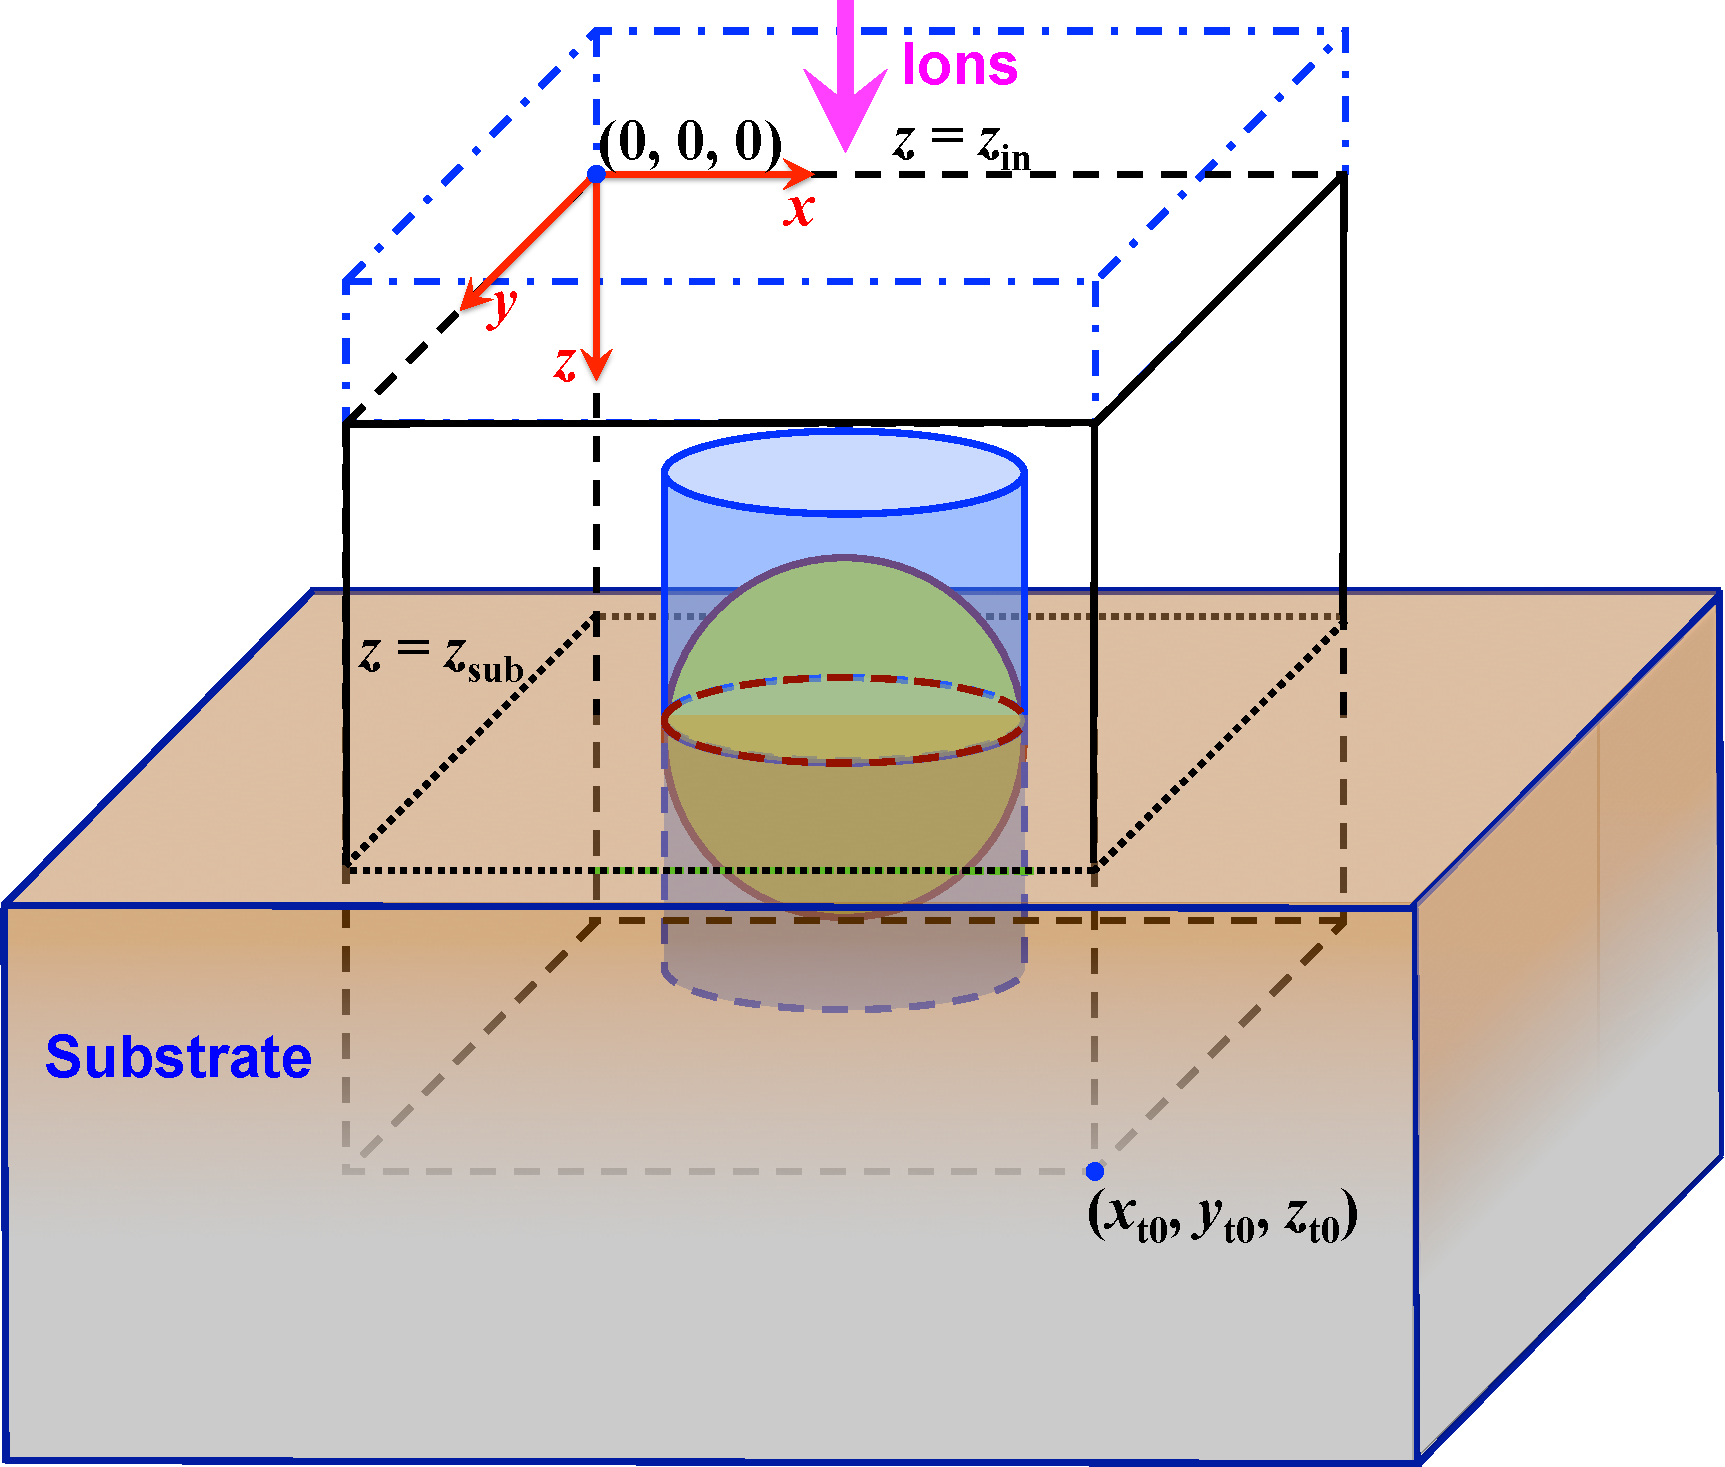
\includegraphics[width=0.48\textwidth]{fig2-a.pdf}
%\label{Fig.1a}
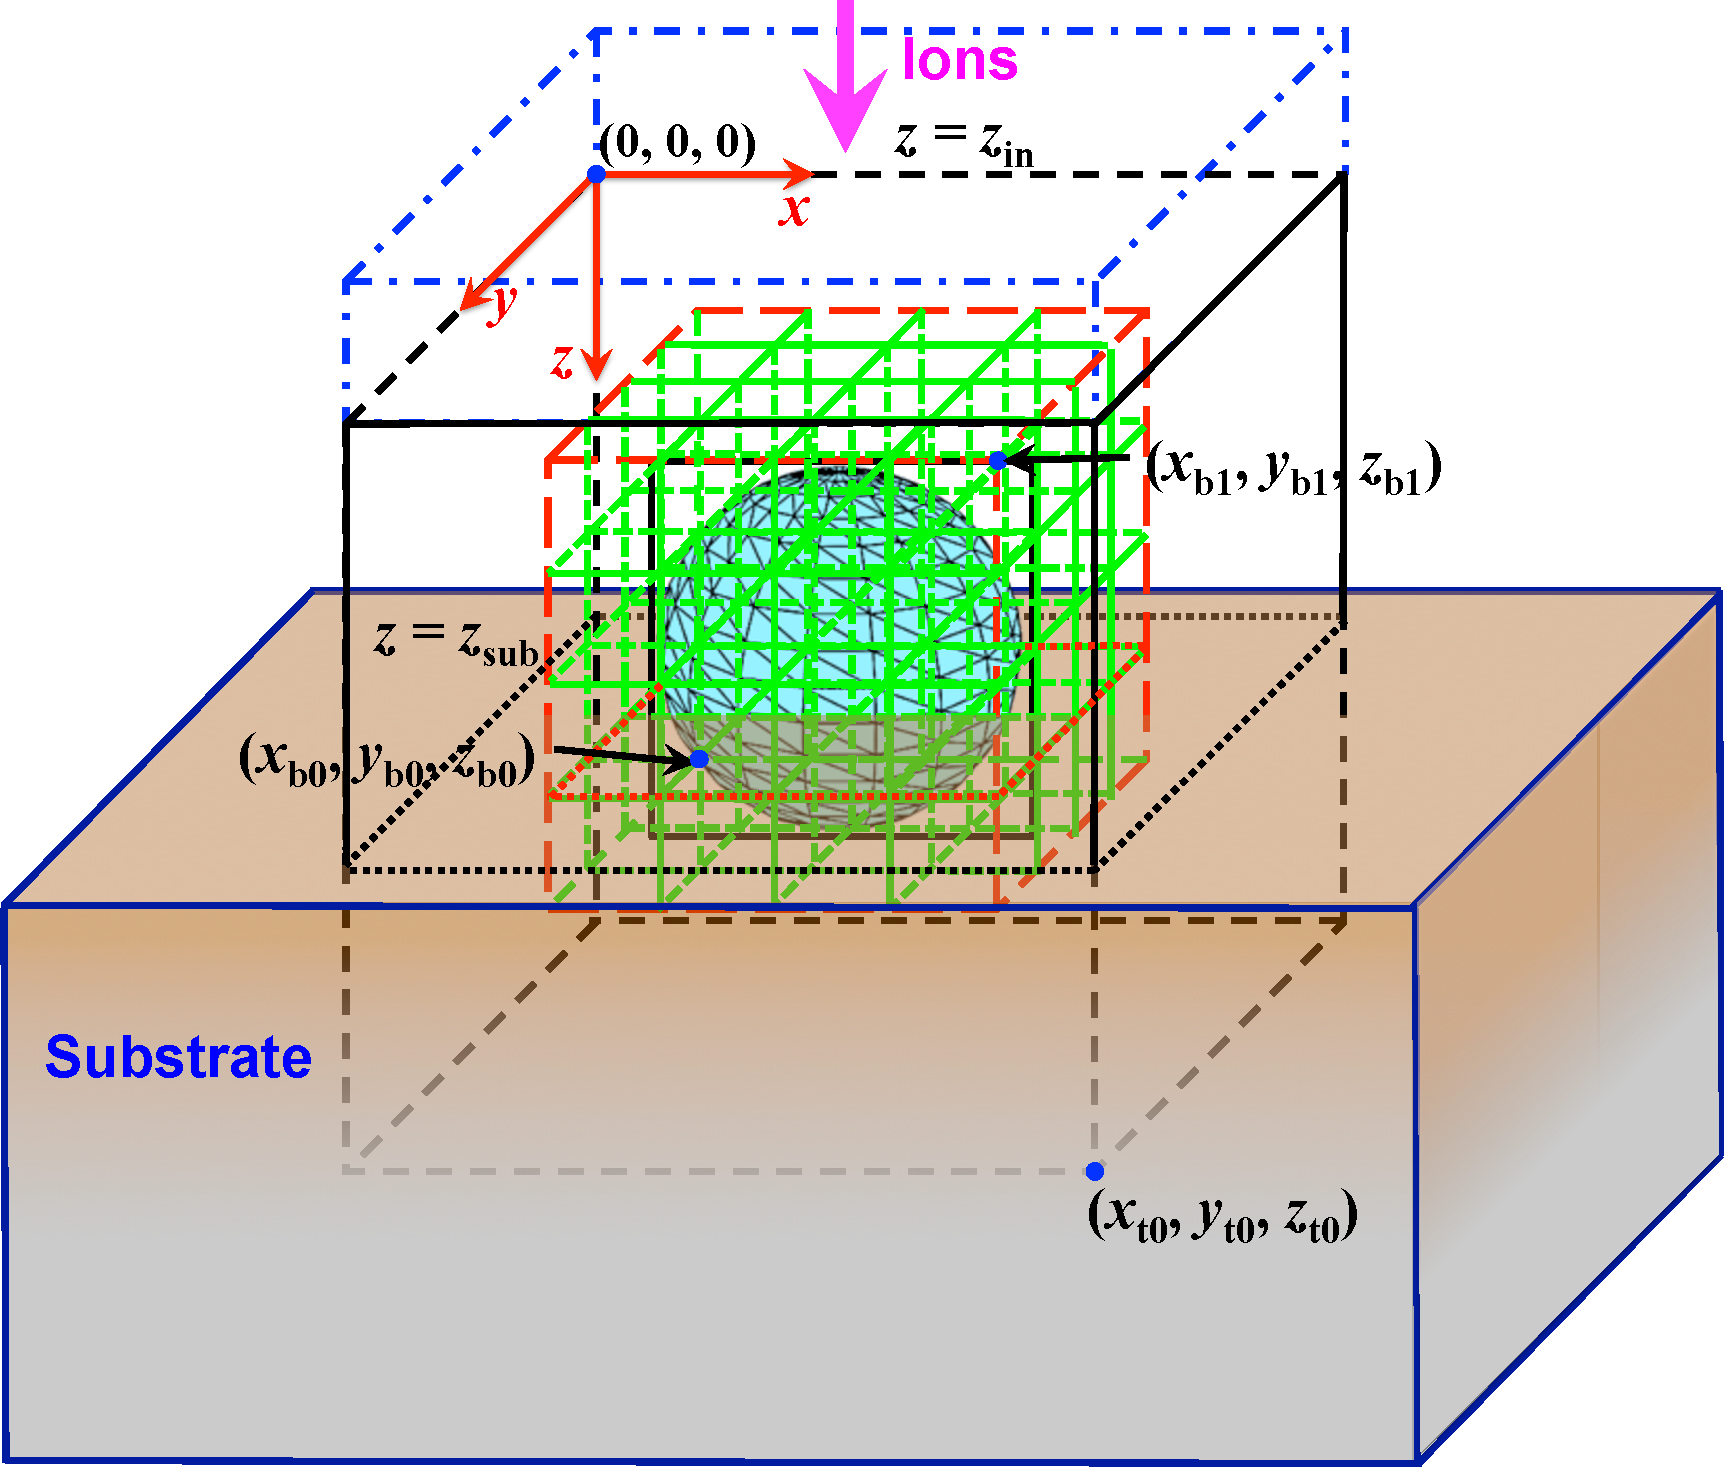
\includegraphics[width=0.48\textwidth]{fig2-b.pdf}
%\label{Fig.1b}
\caption{CSG and FETM geometric models and the corresponding coordinate systems.} \label{Fig.2}
\end{figure}

On the one hand, CSG method\cite{Li:2005,Li:2009} is simply introduced in IM3D code which uses simple geometries to build a complex structure with Boolean operations: union, difference and intersection, etc. By CSG modeling, a complex geometric structure can be constructed with some basic and simple 3D bodies as elements that can be analytically described with a few parameters. The basic elements, such as sphere, tetrahedron, cuboid, ellipsoid, taper, column, polyhedron, paraboloid, hyperboloid and so on, can be easily implemented into subroutines to allow efficient calculation of intersecting points of an ion trajectory with a geometric surface. Detailed construction process can be found in Refs.\cite{Li:2005,Li:2009} . The limits of this method are mainly from two sides: firstly, it is obvious that, with the limited number of parameters, one cannot in practice build an arbitrary-complex geometric structures. Fortunately, most of the simple geometric nanostructures can be modeled by the present algorithm. Secondly, for the step of ion/atom trajectories, one has to compute the intersection points with every possible basic shape. A large number of such judging procedures in a MC simulation would cause a heavy computing cost. An efficient parallel algorithm is needed for the simulation of very complex targets constructing with this geometric model.

On the other hand, FETM method\cite{Li:2008,Zhang:2011} in computer graphics is also employed in IM3D code by using a finite element triangle mesh to construct a sample surface, and furthermore, by using the space subdivision method to accelerate the calculation. In principle, it allows an easy construction of an arbitrary-complex geometric structure with smooth or roughness surface. A closed 3D geometric structure can be constructed by just joining a series of mesh points that outline the 3D geometric structure, which can be generated easily by different algorithms with different graphical softwares (such as Gmsh software\cite{Geuzaine:2009}) or even user's own definition. The accepted formats of FETM shape files are $opengl$ and $ply2$ at present. The reason to use a triangulated mesh is due to its advantage on easier judging of intersection points of a velocity vector with a local triangular plane when considering an ion incidence into a sample surface or emission from a surface. This method is more realistic and unified for simulating much complex targets while on the premise of spending less consuming time.

In IM3D code, the trajectories are traced step by step in a complex 3D target. The free-flight-paths of an ion between two successive collision events follow the Poisson distribution with a mean free-flight-path of $l = n^{(-1/3)}$ (where $n$ is the atomic density of the target) or a constant value specified by user. Afterwards, a ray-tracing technique\cite{Li:2005,Li:2009} for an inhomogeneous specimen with a complex geometric structure and the space subdivision method are introduced to accelerate the calculations\cite{Li:2008,Zhang:2011}. Furthermore, when ions transport in a specimen, three physical quantities, i.e. the free-flight-path, the direction deflection, and the kinetic energy change after refraction at surface/interface, must be treated appropriately, especially at the boundaries of complex geometric structures\cite{Li:2008}.
